\section{学习理论}
\subsection{偏差与方差的权衡}
当在谈及线性回归时,我们在探讨应该用类似$y=\theta_0+\theta_1x$“简单”的模型还是用多项式$y=\theta_0+\theta_1x+\cdots+\theta_x^5$的“复杂”的模型来拟合。我们可以看到如下例子
\begin{center}
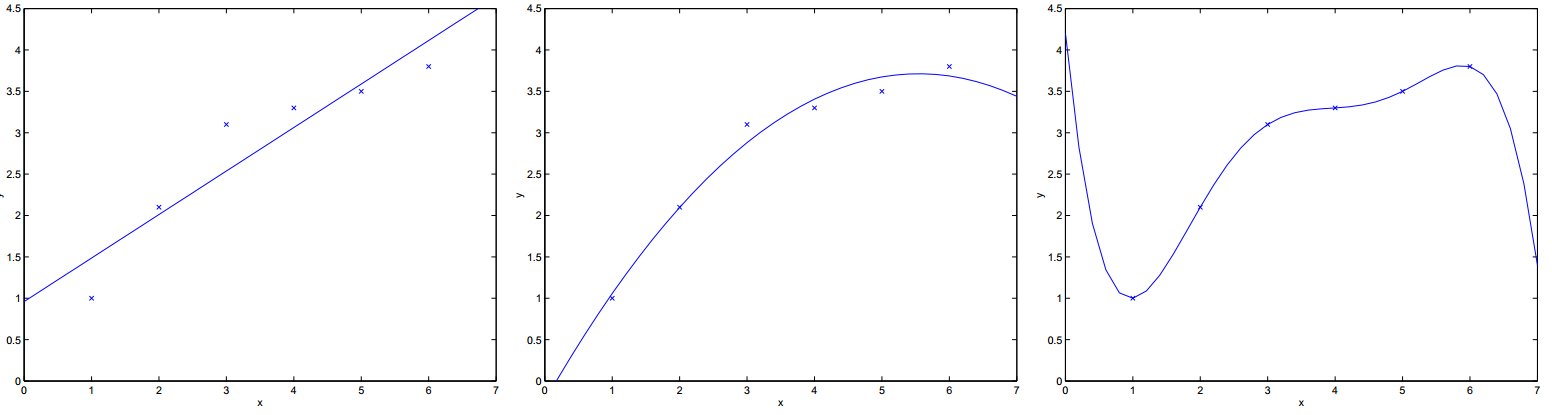
\includegraphics[scale=0.5]{../figures/LT1.PNG} 
\end{center}
拟合5次多项式曲线不是一个好的模型。特殊的,即使是五次的多项式能够很好地从$x$预测$y$,我们还是不认为这个模型十号的。换句话说,这个模型对其他的数据的一般化并不好。我们定义一个假设的泛化误差(generalization error)为该假设的期望风险(error),样本不止来源于训练集。

从上图可以看出,左边的和右边的模型都有较大的泛化误差。然而,这两个模型所遭遇的问题不一样。若$y$与$x$的关系不是线性的,则即使我们有大量的数据,用线性模型去提取数据的特征也会失败。非正式的,我们定义一个模型的偏差(bias)为期望泛化误差。因此,对上面的问题,线性模型有较大的偏差,对于数据可能是欠拟合的情况。

除了偏差,第二个泛化误差的成分为模型拟合的偏差(variance)。特殊的,当像右边的图一样拟合一个五次多项式曲线时,有很大的风险是我们现在提取的数据特征刚好是符合现有的小规模的有限数据集,但是对更大规模的数据并不适用。

因此,经常性的,偏差和方差有权衡。若模型很“简单”,而且具有很少的参数,则其可能会有较大的偏差(但是方差是小的);若模型很“复杂”,而且具有很多的参数,则其可能会有较大的方差(但是偏差是小的)。在以上的例子中,拟合一个二次曲线会比一次曲线和五次曲线这些极端条件要好。

\subsection{引入}
接下来的引理将对下文有所帮助。我们也尝试去探究一些问题:
\begin{itemize}
\item 我们是否可以解决偏差和方差的权衡?
\item 在机器学习中,我们关心泛化误差,但是大部分的算法是根据训练集来训练模型的,为什么我们可以通过训练集来获得关于泛化误差的一些信息呢?特殊的,我们能不能得到训练集的误差和泛化误差的关系?
\item 需要继续什么条件,我们才能证明这个学习算法是好的。
\end{itemize}

\paragraph{引理\ 联合界}假设$A_1,A_2,\cdots,A_k$为$k$个不同的事件,则有
\begin{eqnarray}
P(A_1\cup\cdots\cup A_k)\leq P(A_1)+\cdots+P(A_k)
\end{eqnarray}
在概率理论中,联合界作为公理。

\paragraph{引理\ Hoeffding不等式}假设$Z_1,Z_2,\cdots,Z_m$是$m$个独立同分布(independent and identically distributed(iid))的服从伯努利分布$Bernoulli(\phi)$随机变量,即$P(Z_i=1)=\phi$,$P(Z_i=0)=1-\phi$。$\hat{\phi}$为随机变量的均值,即$\hat{\phi}=\frac{1}{m}\sum_{i=1}^mZ_i$,令$\gamma>0$固定,则有
\begin{eqnarray}
P(|\phi-\hat{\phi}|>\gamma)\leq 2e^{-2\gamma^2m}
\end{eqnarray}
这个引理在学习理论中也被称为Chernoff bound。该引理说明,若用$\hat{\phi}$来估计$\phi$,当$m$增大时,估计值与实际值的距离大于$\gamma$的概率将会被减小。

采用这两个引理,我们可以证明一些比较深层且重要的学习理论结论。

为了简化阐述,我们将目光放在二分类问题,其中标签$y\in\{0,1\}$。假设对于给定的训练集$S=\{(\sample{x}{i},\sample{y}{i});i=1,\cdots,m\}$,其规模为$m$,训练样本$(\sample{x}{i},\sample{y}{i})$服从iid的概率分布$\mathcal{D}$。对于假说$h$,定义训练误差(training error)(在学习理论中也称为经验风险(empirical risk )或经验误差(empirical error )),为如下公式:
\begin{eqnarray}
\hat{\epsilon}(h)=\frac{1}{m}\sum_{i=1}^m1\{h(\sample{x}{i})\neq\sample{y}{i}\}
\end{eqnarray}
可知,只有小部分的$h$的分类错误的数据被使用。对于训练集$S$时记为$\hat{\epsilon}_S(h)$。定义泛化误差(generalization error )为
\begin{eqnarray}
\epsilon(h)=P_{(x,y)\sim D}(h(x)\neq y)
\end{eqnarray}
其表明对于新的服从分布$\mathcal{D}$的数据$(x,y)$,其误分类的概率。

我们假设将要用来估计假说的数据是抽取自同一分布$\mathcal{D}$的,这有时也被作为概率近似正确(PAC(probably approximately correct))的一个设想。

设想一个线性分类,让$h_\theta(x)=1\{\theta^Tx\geq0\}$,一种调节参数$\theta$的方式是最小化训练误差,然后选择
\begin{eqnarray}
\hat{\theta}=\arg\min_\theta\hat{\epsilon}(h_\theta)
\end{eqnarray}
我们将这种方法称为经验风险最小化(ERM(empirical risk minimization )),算法的结果为$\hat{h}=h_{\hat{\theta}}$。我们将ERM看作最“基础”的算法。

为了简化讨论,我们定义假设类(hypothesis class)$\mathcal{H}$为以一种学习算法为基础的所有分类器。比如线性回归,则$\mathcal{H}=\{h_\theta:h_\theta=1\{\theta^Tx\geq 0\},\theta\in \mathbb{R}^{n+1}\}$是所有基于$\mathcal{X}$(输入域)的,判定边界为线性的分类器。

于是ERM可以视为如下式子
\begin{eqnarray}
\hat{h}=\arg\min_{h\in\mathcal{H}}\hat{\epsilon}(h)
\end{eqnarray}

\subsection{有限假设类$\mathcal{H}$的情况}
对于一类学习问题,我们定义假设类$\mathcal{H}=\{h_1,\cdots,h_k\}$,包含了$k$种假设。因此,$\mathcal{H}$为包含有$k$个从$\mathcal{X}$映射到$\{0,1\}$的方程的集合。ERM根据这$k$个方程中训练误差最小来选择$\hat{h}$。

接下来准备考察$\hat{h}$的泛化误差,策略分为两步:
\begin{itemize}
\item 说明对于所有$h$,$\hat{\epsilon}(h)$是$\epsilon(h)$的可靠的估计
\item 说明其中应用了$\hat{h}$的泛化误差的上界
\end{itemize}

任选一个$h_i\in \mathcal{H}$并固定。考虑一个伯努利随机变量$Z$,对于采样$(x,y)\in \mathcal{•}cal{D}$,为$Z=1\{h_i(x)\neq y\}$。类似的,我们定义$Z_j=1\{h_i(\sample{x}{j})\neq\sample{y}{j}\}$。$Z$,$Z_j$对$\mathcal{D}$服从独立同分布。

对于随机的样本的误分类概率,$\epsilon(h)$为$Z$和$Z_j$的期望值。同时,训练误差如下
\begin{eqnarray}
\hat{\epsilon}(h_i)=\frac{1}{m}\sum_{j=1}^mZ_j
\end{eqnarray}
其中,$\hat{\epsilon}(h_i)$为$m$个随机变量$Z_j$的均值,其中,$Z_j$服从均值为$\epsilon(h_i)$的独立同分布的伯努利分布。因此,我们可以应用Hoeffding不等式,得到
\begin{eqnarray}
P(|\epsilon(h_i)-\hat{\epsilon}(h_i)|>\gamma)\leq 2e^{-2\gamma^2m}
\end{eqnarray}

这表明,对于特定的$h_i$,当$m$够大时,训练误差将会很高概率地靠近泛化误差。我们将要证明,这个结论在所有的$h\in\mathcal{H}$同时也成立。令事件$A_i$代表$|\epsilon(h_i)-\hat{\epsilon}(h_i)|>\gamma$。其有性质$P(A_i)\leq 2e^{-2\gamma^2m} $,应用联合界定理,我们求在$\mathcal{H}$中存在$h$,使得$|\epsilon(h_i)-\hat{\epsilon}(h_i)|>\gamma$成立的概率
\begin{eqnarray}
\begin{aligned}
P(\exists h\in \mathcal{H}.|\epsilon(h_i)-\hat{\epsilon}(h_i)|>\gamma ) &= P(A_1\cup\cdots\cup A_k)\\
&\leq \sum_{i=1}^kP(A_i)\\
&\leq \sum_{i=1}^k 2e^{-2\gamma^2m}\\
&= 2ke^{-2\gamma^2m}
\end{aligned}
\end{eqnarray}
求其对立事件,有
\begin{eqnarray}
\begin{aligned}
P(\urcorner(\exists h\in \mathcal{H}.|\epsilon(h_i)-\hat{\epsilon}(h_i)|>\gamma)) &= P(\forall h\in \mathcal{H}.|\epsilon(h_i)-\hat{\epsilon}(h_i)|\leq\gamma )
&\geq 1-2ke^{-2\gamma^2m}
\end{aligned}
\end{eqnarray}

其中,$\urcorner$代表“非”。从上可知,对于所有的$h\in\mathcal{H}$,$\epsilon(h)$和$\hat{\epsilon}(h)$的距离小于$\gamma$的概率至少为$1-2ke^{-2\gamma^2m}$。这被称为一致收敛(uniform convergence),因为这个边界同时适用于所有的$h\in\mathcal{H}$。

记$\delta=2ke^{-2\gamma^2m}$,则对于给定的$\gamma$和$\delta>0$,当$m$取多大时,可以保证概率至少有$1-\delta$,使$\epsilon(h)$和$\hat{\epsilon}(h)$的距离小于$\gamma$?我们可以得到
\begin{eqnarray}
2ke^{-2\gamma^2m} \geq \delta \Rightarrow\ m\geq \frac{1}{2\gamma^2}\log\frac{2k}{\delta}
\end{eqnarray}
其中$\log$又为$\ln$。于是就得到了概率至少为$1-\delta$,对于任意的$h\in\mathcal{H}$,有$|\epsilon(h)-\hat{\epsilon}(h)|\leq \gamma$。这就告诉了我们应该需要多少的训练数据来确保这个界。用来确保算法达到一定的性能的数据大小$m$也被称为算法的样本复杂度(sample complexity)。

上面的界限也有一个重要的结论:样本数据的大小和假设数量$k$为对数关系。

类似的,我们可以固定$m$和$\gamma$,然后求解$\gamma$,对于所有的$h\in\mathcal{H}$,我们可以得到
\begin{eqnarray}
|\hat{\epsilon}(h)-\epsilon(h)|\leq \gamma \leq \sqrt{\frac{1}{2m}\log\frac{2k}{\delta}}
\end{eqnarray}

假定$h^*=\arg\min_{h\in\mathcal{H}}\epsilon(h)$为$\mathcal{H}$中最优的假设,我们有
\begin{eqnarray}
\begin{aligned}
\epsilon(\hat{h})&\leq \hat{\epsilon}(\hat{h})+\gamma\\
&\leq \hat{\epsilon}(h^*)+\gamma\\
&\leq \epsilon(h^*)+2\gamma
\end{aligned}
\end{eqnarray}
对于第一行,是应用了$|\epsilon(\hat{h})-\hat{\epsilon}(\hat{h})|\leq \gamma$。第二行是应用了$\hat{h}=\arg\min_{h\in\mathcal{H}}\hat{\epsilon}(h)$,则有$\hat{\epsilon}(\hat{h})\leq \hat{\epsilon}(h)$都成立,则对于特定的$h^*$,也有$\hat{\epsilon}(\hat{h})\leq \hat{\epsilon}(h^*)$成立。第三行则是再次应用了$|\epsilon(\hat{h})-\hat{\epsilon}(\hat{h})|\leq \gamma$,并将$h^*$代入。于是我们可以得到,当一致收敛性成立,则$\hat{h}$的泛化误差与$\mathcal{H}$中最优的假设的泛化误差只会差$2\gamma$。于是可以得到下面的定理

\paragraph{定理}让$|\mathcal{H}|=k$,令$m,\delta$固定,当训练误差和泛化误差的距离小于一定值的概率至少为$1-\delta$时,我们有
\begin{eqnarray}
\epsilon(\hat{h})\leq \left( \min_{h\in\mathcal{H}}\epsilon(h) \right)+2\sqrt{\frac{1}{2m}\log\frac{2k}{\delta}}
\end{eqnarray}

这证明了当$\gamma=\sqrt{\frac{1}{2m}\log\frac{2k}{\delta}}$,一致收敛性成立的概率至少为$1-\delta$,而且一致收敛性由表明了$\epsilon(h)$最多比$\epsilon(h^*)=\min_{h\in\mathcal{H}}\epsilon(h)$高$2\gamma$。

这也为我们在模型选择中的误差(bias)/方差(variance)权衡中提供了量化。特殊的,假设有一个假设类$\mathcal{H}$,另外假设比$\mathcal{H}'$大很多的假设类,且有$\mathcal{H}'\supseteq\mathcal{H}$。当在$\mathcal{H}'$上考虑问题是,则第一项$\min_{h\in\mathcal{H}}\epsilon(h)$会进一步减小。因此,应用了更大的假设类,则误差(bias)只能减小。然而,若$k$增大,则第二项$2\sqrt{\frac{1}{2m}\log\frac{2k}{\delta}}$将会增大,这对应着当应用更大的假设类时方差(variance)会增大。

像前面所做的,固定$\gamma$和$\delta$,求解$m$,我们可以得到样本复杂度界
\paragraph{推论}让$|\mathcal{H}|=k$,令$\gamma,\delta$固定,为了让$\epsilon(\hat{h})\leq \min_{h\in\mathcal{H}}\epsilon(h)+2\gamma$推出训练误差和泛化误差的距离小于$\gamma$的概率至少为$1-\delta$,需要
\begin{eqnarray}
\begin{aligned}
m&\geq \frac{1}{2\gamma^2}\log\frac{2k}{\delta}\\
&=O\left( \frac{1}{\gamma^2}\log\frac{k}{\delta} \right)
\end{aligned}
\end{eqnarray}

\subsection{无限假设类$\mathcal{H}$的情况}
我们已经得到了关于有限假设类的一些结论。但有很多的假设类,包含了所有的数字(像线性回归),实际上包含了无穷的数字,我们可以得到类似的结论吗?

假设$\mathcal{H}$有$d$个实参数。由于我们用计算机来代表实数,而且双精度是使用64位来代表浮点数,所以假设我们的算法是使用双精度的,于是参数为$64d$位。因此,我们的假设类最多有$k=2^{64d}$种不同的假设。从上一节的推论,为了保证$\epsilon(\hat{h})\leq\epsilon(h^*)+2\gamma$来保证概率至少有$1-\delta$,其需要$m\geq O(\frac{1}{\gamma^2}\log\frac{2^{64d}}{\delta})=O(\frac{d}{\gamma^2}\log\frac{1}{\delta})=O_{\gamma,\delta}(d)$,所以训练集大小最多只与模型的参数数量成线性关系。

事实上我们是依赖了64位精度的条件,这不完全符合所要探讨的条件,但是其结论是大致上正确的。如果我们为了最小化训练误差,为了让含有$d$个参数的假设训练地好,则我们需要和$d$成线性条件的训练数据。

\subsubsection{VC维}
给定假设类$\mathcal{H}$和示例集$D=\{\sample{x}{1},\sample{x}{2},\cdots,\sample{x}{d}\}$,$\mathcal{H}$中每个假设$h$都能对$D$中示例赋予标记,标记结果可表示为
\begin{eqnarray}
h|_D=\{ (h(\sample{x}{1}),h(\sample{x}{2}),\cdots,h(\sample{x}{d}) \}
\end{eqnarray}
随着$d$的增加,$\mathcal{H}$种所有假设对$D$种的示例所能赋予标记的可能结果数也会增大

\paragraph{定义\ 增长函数}对所有$d\in\mathbb{N}$,假设空间$\mathcal{H}$的增长函数$\prod_H(d)$为
\begin{eqnarray}
\prod_\mathcal{H}(m)=\max_{\{ \sample{x}{1},\cdots,\sample{x}{d} \}\subseteq\mathcal{X}}|\{ (h(\sample{x}{1}),h(\sample{x}{2}),\cdots,h(\sample{x}{d})|h\in\mathcal{H} \}|
\end{eqnarray}
增长函数$\prod_\mathcal{H}(m)$表示假设类$\mathcal{H}$对$m$个示例所能赋予标记的最大可能结果数。$\mathcal{H}$对示例所能赋予标记的可能结果数越大,$\mathcal{H}$的表示能力越强,对学习任务的适应能力也越强。因此,增长函数描述了假设空间$\mathcal{H}$的表示能力,由此反映出假设空间的复杂度,我们可利用增长函数来估计经验误差与泛化误差之间的关系

\paragraph{定理}对假设类$\mathcal{H}$,$m\in\mathbb{N}$,$0<\epsilon<1$和任意$h\in\mathcal{H}$,有
\begin{eqnarray}
P(|E(h)-\hat{E}(h)|>\epsilon)\leq 4\prod_\mathcal{H}(2m)e^{-\frac{m\epsilon^2}{8}}
\end{eqnarray}

$\mathcal{H}$中的不同假设对于$D$中示例赋予的结果可能相同,也可能不同。尽管$\mathcal{H}$可能包含无穷多种假设,但其对$D$种示例赋予标记可能结果数是有限的。在一个二分类问题中,最多有$2^m$种结果。$\mathcal{H}$中的假设对$D$中示例赋予标记的每种可能结果称为对$D$的一种“对分”。若假设空间$\mathcal{H}$能实现示例集$D$上的所有对分,即$\prod_\mathcal{H}=2^m$,则称示例集$D$能被假设类$\mathcal{H}$“打散”。

\paragraph{定义\ VC维}假设类$\mathcal{H}$的VC维是能被$\mathcal{H}$打散的最大示例集的大小,即
\begin{eqnarray}
VC(\mathcal{H})=\max\{ m:\prod_\mathcal{H}(m)=2^m \}
\end{eqnarray}
$VC(\mathcal{H})=d$表明存在大小为$d$的示例集能被假设类$\mathcal{H}$打散。若$\mathcal{H}$能打散任意大小的集合,则$VC(\mathcal{H})=\infty$。若存在大小为$d$的示例集能被$\mathcal{H}$打散,但不存在任何大小为$d+1$的示例集能被$\mathcal{H}$打散,则$\mathcal{H}$的VC维是$d$。这就意味着不是多有大小为$d$的示例集都能被假设类$\mathcal{H}$打散,VC维的定义与数据分布$\mathcal{D}$无关。因此,在数据分布未知时仍能计算出假设类$\mathcal{H}$的VC维。

对于下图的数据,我们可以用二分类线性分类器$(h(x)=1\{\theta_0+\theta_1 x_1+\theta_2 x_2\})$所组成的假设类$\mathcal{H}$来打散,为以下八种情况
\begin{center}
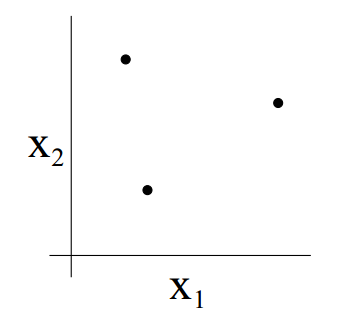
\includegraphics[scale=0.8]{../figures/LT2.PNG} \\
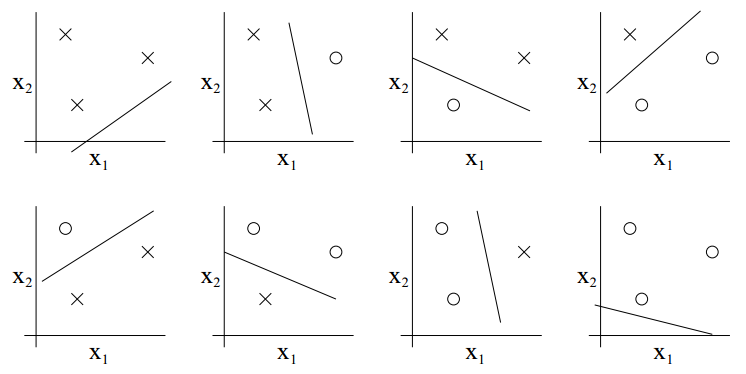
\includegraphics[scale=1]{../figures/LT3.PNG}
\end{center}
由于找不到任何可以被假设类$\mathcal{H}$打散的4个点的数据集,所以$VC(\mathcal{H})=3$。虽然是这样,但有一些三个点的数据是没办法被打散的,比如如下的例子
\begin{center}
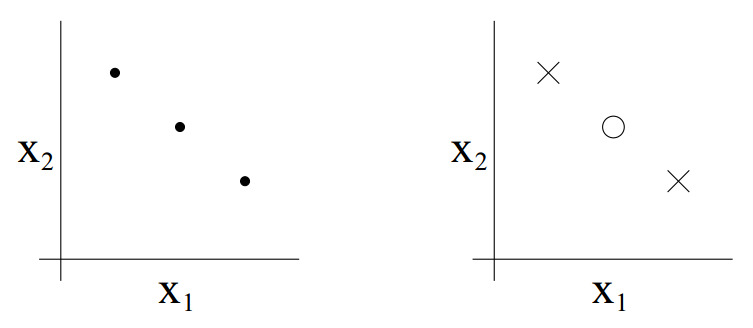
\includegraphics[scale=0.8]{../figures/LT4.PNG}
\end{center}

\paragraph{定理}对于给定的$\mathcal{H}$,且$d=VC(\mathcal{H})$,则为了概率至少能达到$1-\delta$,对于所有的$h\in\mathcal{H}$,有
\begin{eqnarray}
|\epsilon(h)-\hat{\epsilon}(h)|\leq O\left( \sqrt{\frac{d}{m}\log\frac{m}{d}+\frac{1}{m}\log\frac{1}{\delta}}   \right)
\end{eqnarray}
由于概率至少为$1-\delta$,有
\begin{eqnarray}
\epsilon(\hat{h})\leq \epsilon(h^*)+O\left( \sqrt{\frac{d}{m}\log\frac{m}{d}+\frac{1}{m}\log\frac{1}{\delta}}   \right)
\end{eqnarray}
其表明,若一个假设类有有限的VC维,则当$m$增大时,其将一致收敛。于是我们可以得到如下推论

\paragraph{推论}为了$|\epsilon(h)-\hat{\epsilon}(h)|\leq \gamma$来使任意$\in\mathcal{H}$都有概率至少为$1-\delta$,其需要$m=O_{\gamma,\delta}(d)$

这表明,为了让模型能很好的学习,训练集数量需要和$VC(\mathcal{H})$成线性关系。又由于VC维和模型的参数数量成大致的线性关系,因此我们可以得到,训练集所需数量和$\mathcal{H}$的参数数量是成大致的线性关系的。















